\chapter{Understanding source code}

Aesthetics in source code are thus primarily related to cognitive load. In the previous chapter, we've highlighted a focus on understanding when it comes to aesthetic standards: whether obfuscating or illuminating, the process of acquiring a mental model of a given object is a key determinant in the value judgment as applied to source code. In this chapter, we focus on the reason for which such a cognitive load exists in the first place, before surveying the means—both linguistic and mechanistic—that programmers deploy in order to relieve such a load.

This is related to one of the essential features of software: it must be \emph{functional}. As mentioned in our discussion of the differences between source code and software in the introduction, source code is the latent description of what the software will ultimately \emph{do}. Similarly to sheet music, or to cooking recipes\footnote{Recipes are a recurring example taken to communicate the concept of an algorithm to non-experts \citep{zeller_algorithms_2020}}, they require to be put into action in order for their users (musicians and cooks, respectively) to assess their value. Therefore, buggy or dysfunctional software is going to be of less value than correct software \citep{hill_what_2016}, regardless of how aesthetically pleasing the source is.

The assessment of whether a piece of software functions correctly is essentially an assessment of whether what the software does is what the software is supposed to do, which in turn entails knowing what it does, what it is supposed to do, and being able to tell whether these two things are aligned. Any value judgment regarding the aesthetics of the source code at hand would be subject to whether or not the software functions correctly, and such judgment is rendered moot if that software does not work.

After deciding on a benchmark to assess the functionality of the source code at hand (understanding what it should be doing), one must then determine the actual behavior of the source code at hand once it is executed (understanding what it is actually doing). This chapter examines what goes into understanding source code. The first part will lay out our definition of understanding, presenting it as a dual phenomenon, between formalism and contextualism. Starting with 20\^{th} century epistemology, we will see that a dominantly rational, cognitivist perspective on the nature of understanding, as it has been hailed by theoretical computer science research, shows its limits when confronted with practice. Having highlighted this tension, we then turn to how understanding the phenomenon of computation specifically, both on an ontological level, and on a psychological level. The ontological approach will show some of the features of software give it the status on an "abstract artifact", making it a complex object to grasp; the psychological approach will show how such a comprehension takes place for a varity of programmers. Finally, we will conclude with the means that programmers deploy to grasp the concepts at play with software: starting from metaphors used by the general public, we will go down this ladder of abstraction in order to reach the technical apparatuses used in the development and inspection of source code.

The main questions that this chapter addresses are the following: given a certain nature of knowledge acquisition, what are some of the features of computers that make them hard to grasp, and what kind of techniques are deployed in order to address these hurdles and in order to understand what the code is actually doing. This will have us investigate the relationship of knowing and doing, the nature of computation (what is software?) and its relationship to the world as it appears to us (how does modelling and abstraction translate a problem domain into software?), and the cognitive scaffoldings set up to facilitate that task.

% first the definition of understanding
\section{Formal and contextual understandings} %22k char

This section focuses on our definition of understanding—the process of acquiring a working knowledge of an object. Such definition relies on two main aspects: a formal, abstract understanding, and a more subjective, empirical one. We will see how the former had some traction in computer sciences circles, while the second gained traction in programming circles. To support those two approaches, we first trace back the genealogy of understanding in theoretical computer science, before outlining how concrete experience and situatedness outline an alternative tradition.

\subsection{Between formal and informal} %10k

\subsubsection{Theoretical foundations of formal understanding}

To start this inquiry, we go back to the early 20\^{th} century in Cambridge, when the theoretical roots of modern computation were being laid by both philosophers of logic and mathematicians, such as Bertand Russell, Ludwig Wittgenstein, and Alan Turing, as they worked on the formalization of thinking.

Wittgenstein, in particular, bases his argumentation in his \emph{Tractatus Logico-philosophicus} on the fact that much of the problems in philosophy are rather problems of understanding between philosophers—if one were to express oneself clearly, and to articulate one's through clear, unambiguous language, a common conclusion could be reached without much effort:

\begin{quote}
    Most questions and propositions of the philosophers result from the fact that we do not understand the logic of our language. \citep{wittgenstein_tractatus_2010}
\end{quote}

Language and logic are, as we see here, closely connected. Articulated in separate points and sub-points, his work conjugates aphorisms with logical propositions depending on one another, developing from broader statements into more specific precisions. Wittgenstein hints at the intertwining of language as a form of logic, and as logic as a form of language. In this, he follows in the footsteps of Gottfried Leibniz's \emph{Ars Combinatoria}, insofar Leibniz views reasoning and inter-subjective understanding as a formal problem. A universal, and universally-understandable language, called a \emph{characteristica universalis} could resolve any misunderstanding issues. Quoted by Russell, Leibniz notes that:

\begin{quote}
    If we had it [a characteristica universalis], we should be able to reason in metaphysics and morals in much the same way as in geometry and analysis... If controversies were to arise, there would be no more need of disputation between two philosophers than between two accountants [...] Let us calculate. \citep{russell_logical_1950}
\end{quote}

Centuries after Leibniz's declaration, Wittgenstein presents a coherent, articulated theory of meaning through the use of mathematical philosophy, and logic, and his work fits with that of Russell\footnote{In his \emph{Principia Mathematica}, he lays out a theory of logical expression} and Frege\footnote{The \emph{Begriffschrift} similarly attempts to constitute a language in which all scientific statements could be evaluated \citep{korte_frege_2010}, while \emph{Über Sinn und Bedeutung} clarifies the semantic uncertainties between a specific sentence and how it means, or refers to a concept}; even though these are different theories, they are part of a similar endeavour to find a basis od formal propositions through which one could establish truth-values. Such attempt was a direct influence in the work on mathematician Alan Turing—who studied at Cambridge and followed some of Wittgenstein's lectures—, as he developed his own formal system for solving complex, abstract mathematical problems, manifested as a symbolic machine \citep{turing_computable_1936}.

The design of the Turing machine is a subsequent step engagement with the question of understanding in the philosophical sense, as well as in the practical sense—a formal proof to the \emph{Entscheidungsproblem} solved mechanically. Indeed, it is a response to the questions of translation (of a problem) and of implementation (of a solution). This formal approach to instructing machines to operate on logic statements then prompted Turing to investigate the question of intelligence and comprehension in \emph{Computing Machinery and Intelligence}. In it, he translates the hazy term of "thinking" machines into that of "conversing" machines, conversation being a practical human activity which involves listening, understanding and answering (i.e. input, process and output) \citep{turing_computing_2009}. This conversational test, which has become a benchmark for machine intelligence, does rely on the need for a machine to \emph{understand} what is being said. Throughout the article, however, Turing does not yet address the need for a purely formal approach of whether or not a problem can be translated, as Leibniz would have it, into atomistic symbols which would be provided as an input to a digital computer. Such a process of translation would rely on a formal approach, similar to that laid out in the \emph{Tractatus Logico-philosophicus}, or on Frege's formal language described in the \emph{Begriffschrift}. Following a cartesian approach, the idea in both authors is to break down a concept, or a proposition, into sub-propositions, in order to recursively\footnote{although it was not called as such at the time} establish the truth of each of these sub-propositions, and then re-assembled to deduce the truth-value of the original proposition. While Turing focuses on the philosophical and moral arguments to the possibility for machines to think, he does address the issue of artificial intelligence.

With these sophisticated syntactic systems developed a certain approach to cognition, as Turing clearly establishes parallels between the digital computer and the human brain. We now turn to the form of these systems, looking at how their form addresses the problem of clearly understanding and operating on mathematical and logical statements.

Logical calculus, as the integration of the symbol into relationships of many symbols formally takes place through two stylistic mechanisms, the \emph{symbol} and the \emph{list}. Each of the works by Frege, Russell and Wittgenstein quoted above are structured in terms of lists and sub-lists, representing the stylistic pendant to the epistemological approach of related, atomistic propositions and sub-propositions. A list, far from being an innate way of organizing information in humans, is a particular approach to language: extracting elements from their original, situated existence, and reconnecting ways in very rigorous, strictly-defined ways. As Jack Goody writes in \emph{The Domestication of the Savage Mind},

\begin{quote}
    [List-making] [...] is an example of the kind of decontextualization that writing promotes, and one that gives the mind a special kind of lever on 'reality'. \citep{goody_domestication_1977}
\end{quote}

As inventories, early textbooks, administrative documents as public mnemotechnique, the list is a way of taking symbols, pictorial language elements in order to re-assemble them to reconstitute the world, then re-assemble it from blocks, following an assumption that the world can always be decomposed into smaller, discreete and \emph{conceptually coherent} units (i.e. symbols). The list, Goody continues, establishes clear-cut boundaries, they are simple, they are abstract and discontinuous.

Being based on some singular, symbolical entity, applying logical calculus to lists and their symbols, and doing so in a computing environment, becomes the next step in exploring these tools for thinking. Indeed, the engineering development of digital computers in post-war United States as described in \ref{subsec:software-developers}, allowed for the putting into practice of these languages, in the budding field of artificial intelligence (AI).

\subsubsection{Practical attempts at implementing formal understanding}

This putting into practice took the form of subsequent programming languages, relying on a certain conception of human cognition—abstract, logical, as shown above.

IPL, the Information Processing Language, was created by Allen Newell, Cliff Shaw and Herbert A. Simon.  The idea was to make programs understand and solve problems, through "the simulation of cognitive processes" \citep{newell_information_1964}. IPL achieves this with the symbol as its fundamental construct, which at the time was still largely mapped to physical addresses and cells in the computer's memory, and not yet decoupled from hardware.

% add example of IPL
A link between the ideas exposed in the writing of the mathematical logicians and the actual design and construction of electrical machines activating these ideas, IPL was originally designed to demonstrate the theorems of Russell's \emph{Principia Mathematica}, along with a couple of early AI programs, such as the \emph{Logic Theorist}, the \emph{General Problem Solver}. More a proof of concept than a versatile language, IPL was then quickly replaced by LISP as the linguistic means to express intelligence in digital computers.

% add figure on what lisp looks like
LISP (\emph{LIst Processor}) was developed in 1956 was Joseph McCarthy\footnote{McCarthy coined the phrase \emph{Artificial Intelligence} during the 1956 Dartmouth workshop}. The base structural elements of LISP are not symbols, but lists (of symbols, of lists, of nothing), and they themselves act as symbols (e.g. the empty list) \citep{mccarthy_history_1978}. By manipulating those lists recursively—that it, processing something in terms of itself—Lisp shows a tendency for a formal system to separate itself from the problem domain. This is facilitated by its atomistic and relational structure: in order to solve what it has do, it evaluates each symbol and traverses a tree-structure in order to find a terminal symbol, without the explicit need to refer to an external table, for instance.

% add figure on tree structure of language
This sort of heuristic is quite similar to the approach suggested by Noam Chomsky in his \emph{Syntactic Structures}, where he posits the tree structure of language, as a decomposition of sentences until the smallest conceptually coherent parts (e.g. Phrase -> Noun-Phrase + Verb-Phrase -> Article + Substantive + Verb-Phrase). The style is similar, insofar as it proposes a general ruleset (or the at least the existence of one) in order to construct complex structures through simple parts.

Through its direct manipulation of conceptual units upon which logic operations can be executed, LISP became the language of AI, an intelligence conceived first and foremost as logical understanding. The use of LISP as a research tool culminated in the \emph{SHRDLU} program, a natural language understanding program built in 1968-1970 by Terry Winograd which aimed at tackling the issue of situatedness—AI can understand things abtractly through logical mathematics, but can it apply these rules within a given context? The program had the particularity of functioning with a "blocks world" a highly simplified version of a physical environment—bringing the primary qualities of abstraction into solid grasp. The computer system was expected to take into account the rest of the world and interact in natural language with a human, about this world (\emph{Where is the red cube?} \emph{Pick up the blue ball}, etc.). While incredibly impressive at the time, \emph{SHDRLU}'s success was nonetheless relative. It could only succeed at giving barely acceptable results within highly symbolic environments, devoid of any noise. In 2004, Terry Winograd writes:

\begin{quote}
    There are fundamental gulfs between the way that SHRDLU and its kin operate, and whatever it is that goes on in our brains. I don’t think that current research has made much progress in crossing that gulf, and the relevant science may take decades or more to get to the point where the initial ambitions become realistic.  \citep{nilsson_quest_2009}
\end{quote}

This attempt, since the beginning of the century, to enable thinking, clarify understanding and implement it in machines, had first hit an obstacle. The world, also known as the problem domain, exhibits a certain complexity which did not seem to be easily translated into singular, atomistic symbols. Around the same time, however, was developed another approach to formalizing the intricacies of cognition.

Warren McCullough's seminal paper, \emph{A logical calculus of the ideas immanent in nervous activity}, co-written with Walter Pitts, offers an alternative based on the embodiment of cognition. They present a connection between the systematic, input-output procedures dear to cybernetics with the predicate logic writing style of Russell and others \citep{mcculloch_logical_1990}. This attachment to input and output, to their existence in complex, inter-related ways, rather than self-contained propositions is, interestingly, rooted in his activy as a literary critic\footnote{Even at the Chicago Literary book club, he argues for a more sensuous approach to cognition: \emph{"In the world of physics, if we are to have any knowledge of that world, there must be nervous impulses in our heads which happen only if the worlds excites our eyes, ears, nose or skin."} \citep{mcculloch_delusion_1953}}.

Going further in the processes of the brain, he indeed finds out, in another paper with Letvinn and Pitts \citep{lettvin_what_1959}, that the organs through which the world excites the brain \emph{are themselves} agents of process, activating a series of probabilistic techniques, such as noise reduction and softmax, to provide a signal to the brain which isn't the untouched, unary, \emph{symbolical} version of the signal input by the external stimuli, and nor does it seem to turn it into such.

We see here the development of a theory for a situated, embodied stance towards cognition, which would ultimately resurface through the rise of machine learning via convoluted neural networks in the 2000s \citep{nilsson_quest_2009}. In it, the senses are as essential as the brain for an understanding—that is, for the acquisition, through translation, of a conceptual model which then enable deliberate and successful action. It seems, then, that there are other ways to know things than to rely on description through formal propositions.

\vspace*{1\baselineskip}

A couple of decades later, Abelson and Sussman still note, in their introductory textbook to computer science, the difficulty to convey meaning mechanically:

\begin{quote}
    Understanding internal definitions well enough to be sure a program means what we intend it to mean requires a more elaborate model of the evaluation process than we have presented in this chapter. \citep{abelson_structure_1979}
\end{quote}

While formal notation is able to enable digital computation, it nonetheless proved to be limited when it came to accurately and expressively  conveying meaning. This limitation, of being able to express formally what we understand intuitively (e.g. \emph{what is a chair?}\footnote{A question addressed by Joseph Kosuth in his artwork \emph{One and Three Chairs}, 1965}) appeared as computers applications left the domain of logic and arithmetic, and were applied to more social domains.

After having seen the possibilities and limitations of making machines understand through the use of formal languages, and the shift offered by taking into account sensory perception as a possible locus of cognitive processes, we now turn to these ways of knowing that exist in humans in a more embodied capacity.

% todo
% \begin{itemize}
% \item EXAMPLE: XML (applen, mcdaniel, rhetorics of xml)
% \end{itemize}

\subsection{Knowing-what and knowing-how} %10k

1953 saw a radical posture change from one of the logicians whose work underpinned AI research, briefly before the start of these attempts to implement artificial intelligence in digital computers. This was the publication of Wittgenstein's \emph{Philosophical Investigations}. In his second work, he disown his previous approach to language as seen in the \emph{Tractatus Logico-philosophicus}, and favors a more contextual, use-centered frame. Rather than what knowledge is, he looks at how knowledge is acquired and used; while (formal) lanuage was previously defined as the exclusive means to translation concepts in clearly understandable terms, he broadens his perspective in the \emph{Inquiries} by stating that language is \emph{"the totality of language and the activities with which it is intertwined"} and that \emph{"the meaning of a word is its use within language"} \citep{wittgenstein_recherches_2004}, noting context and situatedness as a important factors in the understanding process.

At first, then, it seemed possible to make machines understand through the use of formal languages. The end of the first wave of AI development, as a branch of computation specifically focused on cognition, have shown some limits to this approach.  We now turn to theories which support this approach of an embodied and contextualized knowing, complemented by a constructivist approach to building an understanding.

% 4000
\subsubsection{Knoweldge and situation}

As hinted at by the studies of McCullough and Levitt, understanding a situation doesn't rely exclusively on abstract logical processes, but also on the processes involved in grasping this situation, such as, in their case, peripheral vision processing. It is not just what things are, but how they are, and how they are \emph{perceived}, which matters. Different means of inscription and description do tend to have an impact on the ideas communicated and understood.

In his book \emph{Making Sense: Cognition, Computing, Art and Embodiment}, Simon Penny refutes the so-called unversality of formulating cognition as a formal problem, and develops an alternative history of cognition, akin to Michel Foucault's archeology of knowledge. Drawing on the works of authors such as William James, Jakob von Uexküll and Gilbert Ryle, he refutes the Cartesian dualism thesis which acts as the foundation of AI research \citep{penny_making_2019}. A particular example of the fallacy of dualism, is the use of the phrase \emph{implementation details}, which he recurringly finds in the AI literature, such as Herbert Simon's \emph{The Sciences of the Artificial} \citep{simon_sciences_1996}. The phrase refers to the gap existing between the statement of an idea, of an algorithm, and a procedure, and its concrete, effective and functional manifestation.

For instance, pseudo-code is a way to sketch out an algorithmic procedure, which might be considered agnostic when it comes to implementation details. One can consider the pseudo-code in \ref{code:nielsen_chalktalk}, which describes a procedure to recognize a free-hand drawing and transform it into a known, formalized glyph. Disregarding the implementation details means disregarding any reality of an actual system: the operating system (e.g. UNIX or MSDOS), the input mechanism (e.g. mouse, joystick, touch or stylus), the rendering procedure (e.g. raster or vector), or the programming language (e.g. JavaScript or Python).

\begin{listing}
    \begin{minted}{python}
        recognition = false
        do until recognition
        wait until mousedown
            if no bounding box, initialize bounding box
            do until mouseup
            update image
            update bounding box
            rescale the material that's been added inside
            if we recognize the material:
                delete image from canvas
                add the appropriate iconic representation
                recognition = true
    \end{minted}
    \caption[]{Example of pseudo-code attempting to reverse-engineer a software system, ignoring any of the actual implementation details, taken from \citep{nielsen_working_2017}}
    \label{code:nielsen_chalktalk}
\end{listing}

Refuting the idea that pseudo-code is all that is necessary to communicate and act upon a concept, Penny  argues on the contrary that information is relativistic and relational; relative to other pieces of information (intra-relation) and related to contents and forms of presenting this relation (extra-relation). Pseudo-code will only ever make sense in a particular implementation context, which then affects the product.

He then follows Philip Agre's statement that a theory of cognition based on formal reason works only with objects of cognition whose attributes and relationships can be completely characterized in formal terms; and yet a formalist approach to cognition does not prove that such objects exist or, if they exist, that they can be useful. Uses of formal systems in artificial intelligence in specific, and in cognitive matters in general, is yet another instance of the map and the territory problem—it only goes so far.

Beyond the syntax of formal logic, there are different ways to transmit cognition in actionable form, depending on the form, the audience and the purpose. In terms of form, a symbol system of formal logic is only one of many possibilities for systems of forms. In his \emph{Languages of Art}, Nelson Goodman elaborates a theory of symbol systems, which he defines as formal languages composed of syntactic and semantic rules \citep{goodman_languages_1976}. Logical notation exists along with music, painting, poetry and prose. What follows, argues Goodman, is that all these formal languages involve an act of \emph{reference}. Through different means (exemplification, denotation, resemblance, representation), formal systems act as sets of symbols which can denote or exemplify or refer to in more complex and indirect ways, yet always between a sender and a receiver\footnote{Understood as the eponymous entities  in Jakobsen's model of communication functions.}.

Communication, as the transfer of meaning from one individual to one or more other individuals, does not exclusively rely on the use of mathematical based use of formal languages. From Goodman to Goody, the format of representation also affords differences in what can be thought and imagined. Something that was always implicit in the arts—that representation is a complex and ever-fleeting topic—is shown more recently in Marchand-Zañartu and Lauxerois's work on pictural representations made by philosophers, visual artists and novelists (such as Claude Simon's sketches for the structure of his novel \emph{La Route des Flandres}, shown in \ref{image:routedesflandres}) \citep{marchand-zanartu_32_2022}. How specific domains, from mathematics to visual arts and construction, engage in the relation between form and cognition is further adressed in CHAPTER\_4.

\begin{figure}
    \begin{center}
        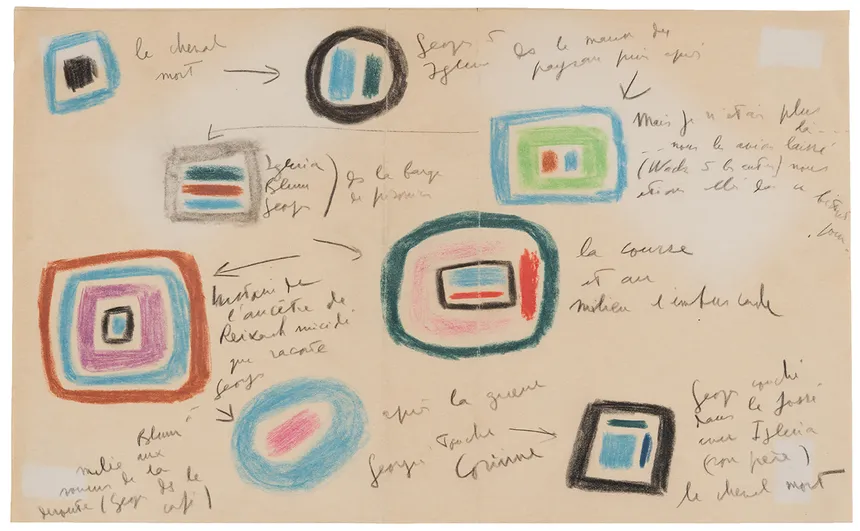
\includegraphics[width=\textwidth,height=\textheight,keepaspectratio]{routedesflandres.png}
        \caption{Tentative d'organisation visuelle pour le roman La Route des Flandres, années 1960 - Claude Simon, écrivain}
        \label{image:routedesflandres}
    \end{center}
\end{figure}

Going beyond logical notation, we have seen that there are other conceptions of knowledge which take into account the physical, social and linguistic context of an action. Nonetheless, these can still be systematized, as Goodman highlights in his investagation of referential systems, with a focus on reference of the ideas at hand.

% 4000
\subsubsection{Constructing knowledge}

There are multiple ways to express an idea: on can use formal notation or draft a rough sketch with different colors. These all highlight different degrees of expression, but one particular way can be considered problematic in its ambition. Formal languages rely on the assumption, that all which can be known can ultimately be expressed in unambiguous terms. First shown by Wittgenstein in the two main eras various eras of his work, we know focus on the ways of knowing which cannot be explicited.

First of all, there is a separation between \emph{knowing-how} and \emph{knowing-that}; the latter, propositional knowledge, does not cover the former, practical knowledge, as shown by Ryle \citep{ryle_concept_1951}. Perhaps one of the most obvious example of this duality is in the failure of Leibniz to construct a calculating machine, as told by Matthew L. Jones in his book \emph{Reckoning with Matter}. In it, he traces the history of philosophers to solve the problem of constructing a calculating machine, a problem which would ultimately be solved by Charles Babbage, with the consequences that we know \citep{jones_reckoning_2016}.

Jones depicts Leibniz in his written correspondence with watchmaker Ollivier, in their fruitless attempt to construct Leibniz's design; the implementations details seem to elude the German philosopher as he refers to the "confused" knowledge of the nonetheless highly-skilled Parisian watchmaker. The (theoretical) plans of Leibniz do not match the (concrete) plans of Ollivier.

These are two complementary approaches to the knoweldge of something: to know \emph{what} constructing calculating machine entails and knowing \emph{how} to construct such a machne. In the fact that Ollivier could not communicate clearly to Leibniz what his technical difficulties, we can see an instance of something which would be theorized centuries later by Michael Polanyi as \emph{tacit knowledge}, knowledge which cannot be entirely made explicit.

Polanyi, as a scientist himself, starts from another assumption: we know more than we can tell. In his eponymous work, he argues against a positivist approach to knowledge, in which empirical and factual deductions are sufficient to achieve satisfying epistemological work. What he proposes, derived from \emph{gestalt} psychology, is to consider some knowledge of an object as the knowledge of an integrated set of particulars, of which we already know some features, by virtue of the object existing in an external approach. This integrated set, in turn, displays more properties than the sum of its parts. While formal notation suggests that the combination of formal symbols does not result in additional knowledge, Polanyi rather argues, against Descartes, that relations and perceptions do result in additional knowledge.

\begin{quote}
    The knowledge of a problem is, therefore, like the knowing of unspecifiables, a knowing of more than you can tell. \citep{polanyi_knowing_1969}
\end{quote}

Rooted in psychology, and therefore in the assumption of the embodimed of the human mind, Polanyi posits that all thought is incarnate, that it lives by the body and by the favour of society, hence giving it a physio-social dimension. This confrontation with the real-world, rather than being a strict hurdle that has to be avoided or overcome, as in the case of SHRDLU above, becomes one of the two poles of cognitive action. Knowledge finds its roots and evaluation in concrete situations, as much as in abstract thinking. In the words of Cecil Wright Mills, writing about his practice as a social scientist research,

\begin{quote}
    Thinking is a continuous struggle between conceptual order and empirical comprehensiveness. \citep{MillsC.WrightCharlesWright2000Tsi}
\end{quote}

Polanyi's presentation of a form of knowledge following the movement of a pendulum, between dismemberment and integration of concepts finds an echo in the sociological work of Mills: a knowledge of some objects in the world happens not exclusively through formal descriptions in logical symbol systems, but involves imagination and phenomenological experience—wondering and seeing. This reliance on vision—starting by recognizing shapes, as Polanyi states—directly implies the notion of aesthetic assessment, such as a judgement of typical or non-typical shapes. He does not, however, immediately elucidate how aesthetics support the formation of mental models at the basis of understanding, only that this morphology is at the basis of higher order of represenations.

Seeing, though, is not passive seeing, simply noticing. It is an active engagement with what is being seen. Mills's quote above also contains this other aspect of Polanyi's investigation of knowledge, and already present in Ollivier's relation with Leibniz: knowing through doing.

This approach has been touched upon from a practical programmer's perspective in section \ref{subsec:craft-knowledge}, through a historical lens but it does also posses theoretical grounding. Specifically, Harry Collins offers a deconstruction of the Polanyi's notion by breaking it down into \emph{relational}, \emph{somatic} and \emph{collective} tacit knowledges \citep{collins_tacit_2010}. While he lays out a strong approach to tacitness of knowledge (i.e. it cannot be communicated at all), his distinction between relational and somatic is useful here\footnote{His definition of collective tacit knowledge touches on the knowledge present in any living species and is impossible to ever be explicited, and is therefore out of scope here.}. It is possible to think about knowledge as a social construct, acquired through social relations: learning the linguo of a particular technical domain, exchanging with peers at conferences, imitating an expert or explaining to a novice. Collective, unspoken agreements and implicit statements of folk wisdom, or implicit demonstrations of expert action are all means of communication through which knowledge gets replicated across subjects.

Concurrently, somatic tacit knowledge tackles the physiological perspective as already pointed out by Polanyi. Rather than knowledge that exists in one's interactions with others, somatic tacit knowledge exists within one's physical perceptions and actions. For instance, one might base one's typing of one's password strictly on one's muscle memory, without thinking about the actual letters being typed, through repetition of the task. Or one might be spotting a cache bug which simply requires a machine reboot, due to experience machine lifecycles, package updates, networking behaviour. Not completely distinct from its relational pendant, somatic knowledge is acquired through experience, repetition and mimeomorphism—replicating actions and behaviours, or the instructions, often under the guidance of someone more experienced.

\vspace*{1\baselineskip}
\centerline{\rule{0.13334\linewidth}{.4pt}}
\vspace*{1\baselineskip}

We started our discussion of understanding by defining it as the acquisition of the knowledge of a object—be it a concept, a situation, an individual or an artfefact,, which is accurate enough that it allows us to predict the behaviour and to interact with such object. Within this defintion, one could take the example of a human discussion as a demonstration of advanced understanding, as something that is both situated, and formalized.

Theories of how individuals acquire understanding (how they come to know things, and know conceptual representations of things), have been approached from an explicit perspective, and an implicit one. In the rationalist, logical philosophical tradition, we have seen that the belief that meaning can be rendered unambiguous through the use of specific notation. This has led to the development of logic and computer science, as this meaning got mechanized. Explicit understanding is therefore the theoretical lineage of computation.

However, as we've seen in the first hurdles of artificial intelligence research, explicit specification of meaning falls short of handling everyday tasks which humans would consider to be menial. This has led us to consider a more implicit approach to understanding, in which it is acquired by tacit means. Particularly, we've identified this tacit knowledge as relying on a social component, as well as on a somatic component.

Source code, as a formal system with a high dependence of context, intent and implementation, mobilizes both approaches to understanding. Before we dive deeper about how these two modes of understanding are mobilized at the end of this chapter, we now turn to what makes computation a cognitively complex object, and what are some cognitive reactions that humans display in situations where they have to understand, and work with, software.

\clearpage

% first the computer
\section{Understanding computation}

In the previous chapter, we've laid out the groundwork by showing that there are multiple ways to understand something. We now turn to the thing we want to understand. What makes it challenging to understand computation?

First, we will inquire into some distinguishing features of software, by looking at some of its particularities, in terms of levels of abstractions, and in terms of types of complexity. This will highlight some of the theoretical properties that make it hard to understand, such as its relation to hardware, its relation to a specification, and its relation to time and space.

Then, we will shift our perspective to a more abstract point of view, investigating the ontological status of software. This will highlight how software exists as an \emph{abstract artifact}, a term which encapsulates software's intrinsic and extrinsic tensions.

Finally, we will conclude this section by looking specifically at the source code component of software, and how programmers deploy strategies to understand it. Approaching it from a cognitive and psychological perspective, this will give us a better picture of the concrete process of understanding source code—a process which aesthetics are primarily intended to affect.

% the software effect (combination of knowing what (it does) and how (it does it))
\subsection{Software complexity} %7k

Software exhibits several particularities, which result in a compex whole—meaning that software possesses several independent components which interact with each other in non-trivial, and non-obvious ways. This subsection focuses on these particularies; that is, on the \emph{properties} of software, and hence how these properties manifest themselves concretely, leading to those complex interactions. We will start by looking at the different levels at which software exists, before turning to the different kinds of complexity which make software hard to grasp.

\subsubsection{Levels of software} % 3k

One of the essential aspects of software is that of \emph{implementation}. Implementation is the realization of a plan, the concrete manifestation of an idea, and therefore hints at a first tension in software's multiple facets. It can happen through individuation, instantation, exemplification and reduction \citep{rapaport_philosophy_2005}. On the one side, there is what we will call here \emph{ideal} software, often existing only as a shared mental representation by humans (not limited to programmers), or as printed documentation, as a series of specifications, etc. On the other side, we have \emph{actual} software, which is manifested into lines of code, written in one or more particular languages, and running with more or less bugs.

The relationship between the \emph{ideal} and the \emph{actual} versions of the same software is not straightforward. Ideal software only provides an intent, a guidance towards a goal, assuming, but not guaranteeing, that this goal will be reached. A popular engineering saying is that complements this approach by stating that:

\begin{quote}
    In theory, there is no difference between theory and practice. In practice, there is.\footnote{Sometimes mis-attributed to Richard P. Feynman or Albert Einstein, but traced to Benjamin Brewster, writing in the Yale Literary Magazine of 1882.}
\end{quote}

Actual software, as most programmers know, differs greatly from its ideal version, largely due to the process of implementation, translating the purpose of the software from natural and diagrammatic languages, into programming languages, from what it should do, into what it actually does.

Writing on the myths of computer science, James Moor \citep{moor_three_1978} allows us to think through this distinction between ideal and practical along the lines of the separation between a theory and a model. The difference between a model and a theory is that both can exist independently of one another—one can have a theory for a system without being able to model it, while one can also model a system using \emph{ad hoc} programming techniques, instead of a coherent theory.

Most of the practice of programmers (writing and reading code for the purposes of creating, maintaining and learning software) depends on closing this gap between the ideal and the practical existences of software.

The third level at which software exists is that of hardware. While the ideal version of software is presented in natural language, diagrams or pseudo-code, and while the practical version of software exists as executable source code, software also exists at a very physical level—that of transistors and integrated circuits.

The distinction between software and hardware has been examined thoroughly \citep{kittler_there_1997,chun_sourcery_2008,rapaport_philosophy_2005}, but never strictly defined. Rather, the distinction between what is hardware and what is software is relative to where one draws the line: to a front-end web developer writing JavaScript, the browser, operating system and motherboard might all be considered hardware. For a RISC-V assembly programmer, only the specific CPU chip might be considered hardware, while the operating system being implemented in C, itself compiled through Assembly, would be considered software. A common definition of hardware, as the physical elements making up the computer system, overlooks the fact that software itself is, ultimately, physical changes in the electrical charge of the components of the computer.

Software can be characterized the dynamic evolution of logical processes, described as an ideal specification in natural languages, as a practical realization in programming languages, and in specific states of hardware components. Furthermore, the relations between each of these levels is not straightforward: the ideal and the practical can exist independently of each other, while the practical cannot exist independently of a machine\footnote{Even if that machine is a \emph{virtual machine}, further complicating the boundary between hardware and software}.

\subsubsection{Types of complexity} % 4k

Along with different levels of existence needed to be taken into account by the programmer, software also exhibits specific kinds of complexity. Our definition of complexity will be the one proposed by Warren Weaver. He defines problems of (organized) complexity as those which involve dealing simultaneously with a sizable number of factors which are interrelated into an organic whole \citep{weaver_science_1948}\footnote{As opposed to disorganized complexity, which are dealt with statistical tools.}. Specifically, there are four different types of software complexity that we look at: conceptual complexity, modeling complexity, temporal complexity and spatial complexity.

Conceptual complexity, as refered to by Lando et. al. in their ontology of computer programs, addresses the necessity to model complex objects at different abstraction levels \citep{lando_general_2007}. As mentioned above, software exists at least on three somewhat distinct levels: the ideal, the practical, and the physical. This means that software, in its source code representation, should be able to provide the programmer with tools to engage with its intended function and its actual function at each of these levels. For instance, comments might relate to the ideal behaviour of the software, function declarations to its practical behaviour, while macro definitions can point to the specific hardware on which the code is run.

% insert a table of C code where you see some comment, some function, and some macro

Additionally, conceptual complexity involves the distinction of the different elements of a computer program at the source code level, and keep track of their ontological status, sometimes independently from its level of existence. This distinction should be made notwithstanding the naming conventions assigned by different platforms, vendors, or programming languages, and rather based on ontological properties of the elements at hand. For instance, the distinction between \emph{endurants} and \emph{perdurants} by Lando et. al. focuses on the temporal dimension of software components (i.e. a data structure declaration has a different temporal property than a function call). Here we have a second, complementary frame to that of the levels of existence, through which we can analyze source code; being somewhat related but an exact mapping of one another.

Modeling complexity addresses the hurdles in translating a non-discrete, non-logical object, event, or action, into a discreete, logical software description through source code. Indeed, the history of software development is also the history of the extension of the application of software, and the hurdles to be overcome in the process. From translation of natural languages \citep{poibeau_machine_2017}, to education \citep{watters_teaching_2021} or psychological treatment \citep{weizenbaum_computer_1976}, it seems that problems that seem somehat straightforward from a human perspective become more intricate once the time for implementation has come.

We've seen so far the complexities tied to the conceptualization and modelization of the components of software. Two other significant contributions to the cognitive load of understanding software happen are more closely related to the concrete execution of the software—temporal and spatial complexity.

Temporal complexity relates to the discrepancy between the original conceptualization of the computer as a Turing machine—i.e. a machine which operates linearly, on a one-dimensional tape—and further technological developments. Originally, the Turing machine would involve the ability for the head of the machine to jump at different locations. This meant that the execution and reading of a program would be non-linear, jumping from one routine to another across the source code. Such an entanglement is particulary obvious in Ben Fry's Distellamap series of visualizations of source code (\ref{graphic:pacman-visualization} represents the execution of the source code for the arcade game Pac-Man), and led to Edsger W. Dijkstra's statement on the harmfulness of such jumps on the cognitive abilities of programmers.


\begin{listing}
    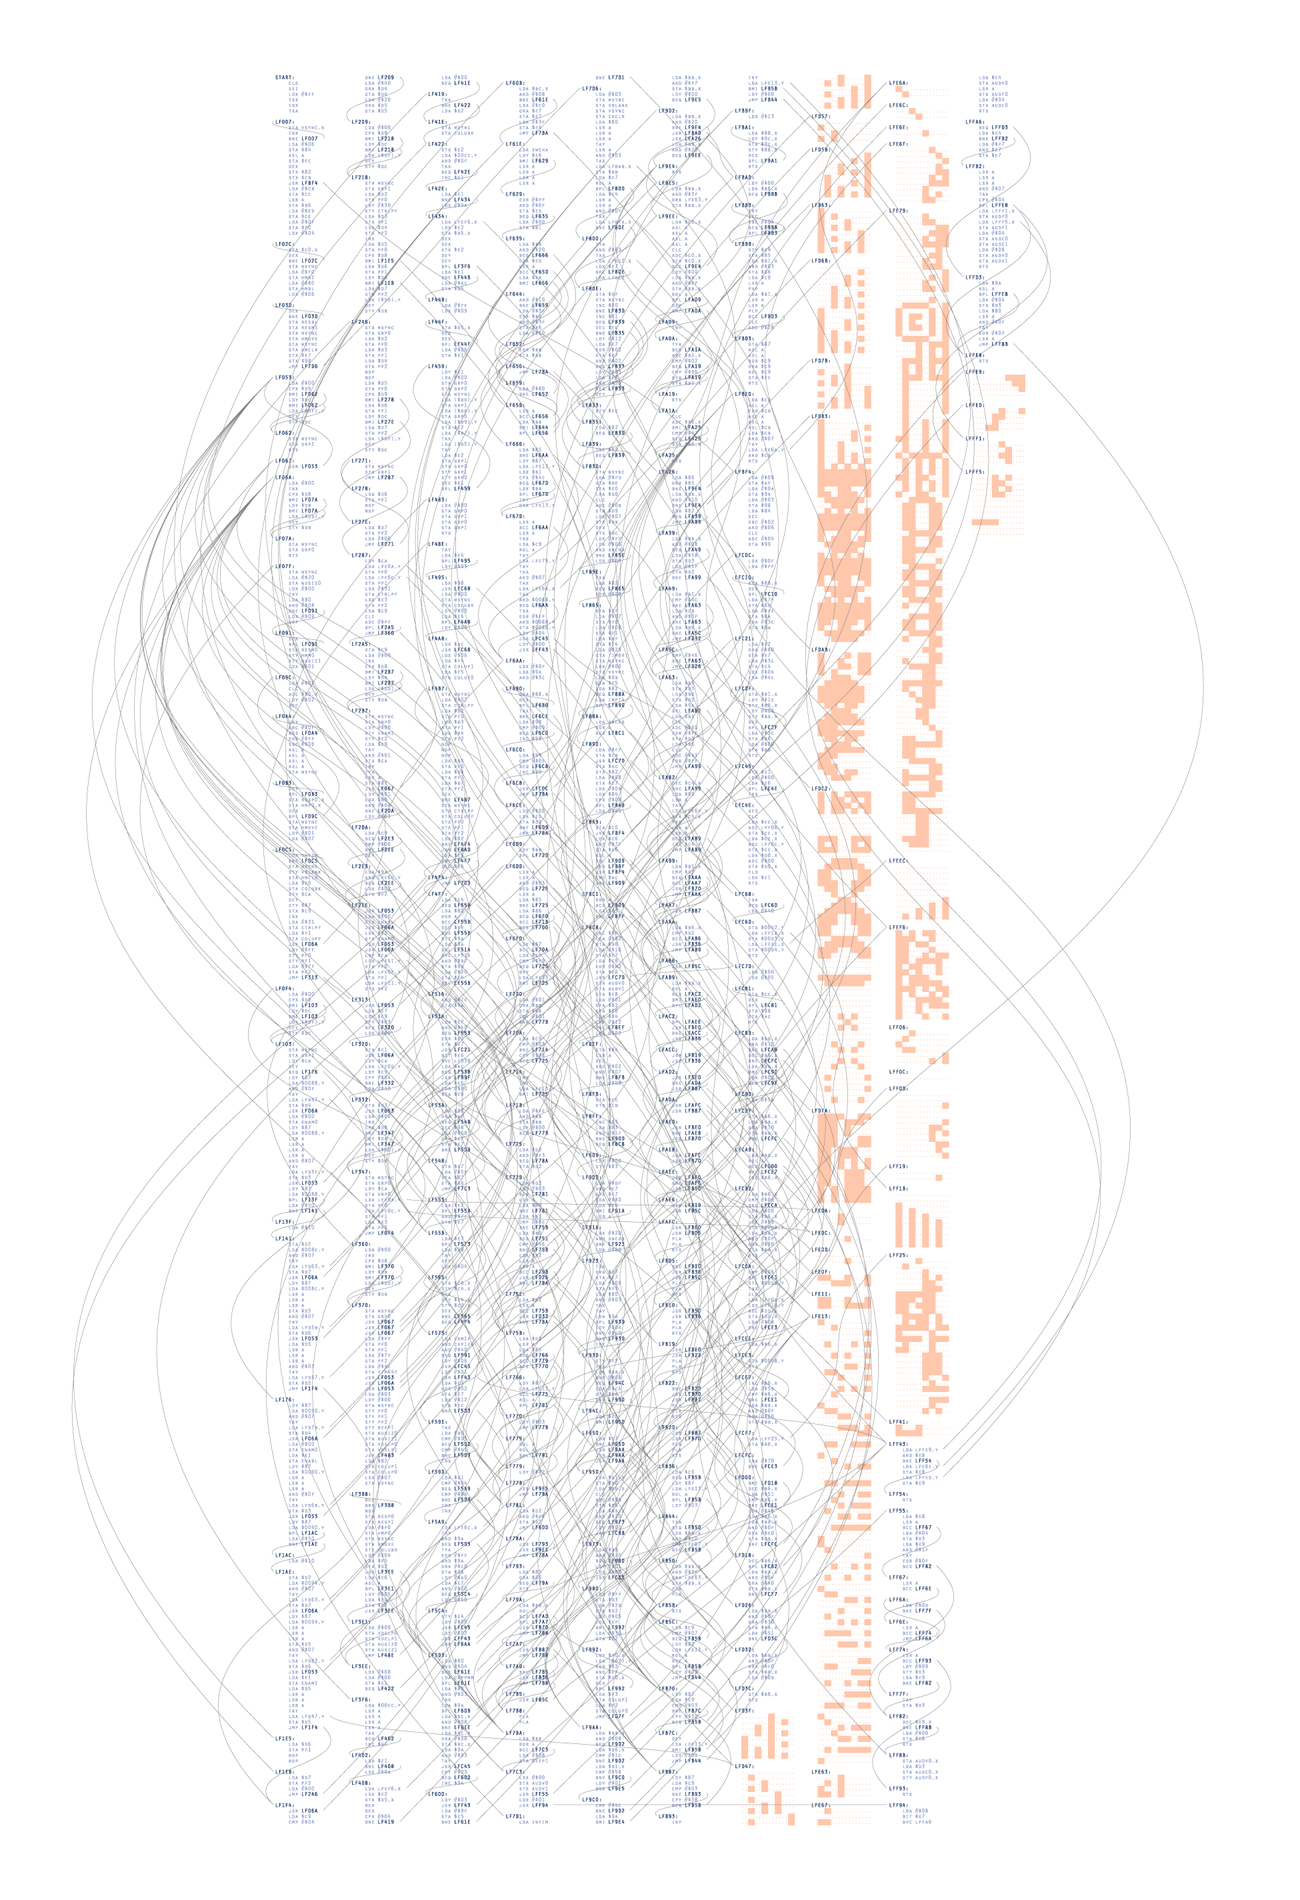
\includegraphics[width=\textwidth,height=\textheight,keepaspectratio]{distellamap_pacman.png}
    \caption{Visualization of the execution of Pac-Man's source code}
    \label{graphic:pacman-visualization}
\end{listing}

Later on, the introduction of multi-core architecture for central processing units in the late 2000s has enabled the broad adoption of multithreading and threaded programming. As a result, source code has transformed from a single non-linear execution to a multiple non-linear process, in which several of these non-linear executions are happening in parallel. Keep tracking of what is executing when on which resource is involved in problems such as \emph{race conditions}, when understanding the scheduling of events (each event every e.g. 1/18000000th of a second on a 3.0 Ghz CPU machine) becomes crucial to ensuring the correct behaviour of the software.

Conversely, the locus of the execution of software creates contributes to those issues. Software can be (dis-)located across multiple files on a single machine, on multiple processes on a single machine, or on multiple processes on multiple machines (on a local-area or wide-area network) \citep{berry_philosophy_2011}. This further fragments the interface to the object of understanding. For instance, the asynchronicity of requesting and processing information from distinct processes is a spatial separation of code which has temporal implications (e.g. due to network latency).

\vspace*{1\baselineskip}
\centerline{\rule{0.13334\linewidth}{.4pt}}
\vspace*{1\baselineskip}

Software, then, exhibits certain properties which make it difficult to understand, from conception to application: software in the real-world involves implementing concepts that lose in translation, interfacing the world through discreete representations, and following the execution of these representations through space and time, as software executes more and more in a distributed and parallel fashion.

% the philosophical enquiries
\subsection{Software ontology} %7k

Now that we've clarified some difficulties in the understanding of software, we can frame these difficulties in a philosophical context. It turns out that not only is the nature of software a complex philosophical object, but so is that of computer science. Computer science itself inherits this complexity from the nature of technology itself. Before moving back to practical inquiries into how specific individuals engage with this nature, this section will help provide a theoretical backdrop for further empirical inquiries. This conceptual framework will first by an investigation into the denomination of software as an \emph{abstract artifact}, followed by an analysis of the ambiguous status of computer science between a science and a technology.

% first on the abstract artifact - 3.5k
\subsubsection{Software as abstract artifact}

When he coins the phrase \emph{abstract artifact}, Nurbay Irmak addresses software as an abstract object, similar to Platonic entities, but have nonetheless have spatio-temporal properties \citep{irmak_software_2012}. As mentioned previous, software does need to exist as an implementation, in the form of source code \citep{suber_what_1988}; this implies that software has a begin and an end, all the while representing ideas of structure and procedure which go beyond this beginning and end. Typically, the physical aspects of software (its manifestation as source code) can be changed\footnote{A process called \emph{refactoring}.} without changing any of the ideas expressed by the software—a phenomenon one can also observe in natural languages, in which one can radically change a syntax without drastically changing the semantics of a sentence.

Colburn's phrasing is that of a \emph{concrete abstraction}. He does not explicit this dichotomy further, but we can see how its oxymoronic nature resonates with the concept of an abstract artifact.

He grounds this tension in the distinction between a medium of execution (a—potentially virtual—machine) and a medium of description (source code). He considers that while, ultimately, any high-level language in which the programmer writes is already the result of layers of abstraction, such high-level language gets reduced to the zeroes and ones input into the central processing unit \citep{colburn_philosophy_2000}. And yet, if we carry on this reasoning further, these representation of voltage changes into zeroes and ones are themselves abstractions over a concrete, physical event.

Writing on computational artefacts, of which software is a subset, Raymond Turner formalizes this apparent contradiction in a three-way relationship. Namely, artefact A is an implementation in medium M of the definition F. For instance, concerning the medium:

\begin{quote}
    Instead of properties such as \emph{made from carbon fiber}, we have properties such as \emph{constructed from arrays in the Pascal programming language, implemented in Java}. \citep{turner_computational_2018}
\end{quote}

This metaphor provides an accurate account of the place of source code within the definition of software: source code is that which gives the ideas in software shape—through a process of concretization—and which hides away the details of the hardware—through abstraction.

The concept of \emph{abstract artifact} therefore helps to clarify the tensions within software, and to locate the specific role of source code within the different moving parts of definition, medium and model.

Software, as a part of the family of technical artefacts, has \emph{functional} properties (i.e. purpose that are intended to be achieved through their use) and \emph{structural} ones (physical configuration which are involved in the fullfilment of the functional purpose) \citep{turner_computational_2018}. As it turns out, these tensions exist throughout computer science and technology as a whole.

\subsubsection{Philosophical investigations into software} %3.5k

The fact that software exists between the state of being conceptually designed and materially implemented predates software itself, and can be observed in modern technological developments at large.

As we've seen, software exists at the intersection of various tensions, domains and perspectives. According to Gilbert Simondon, the technical object is a relation between multiple structures and a complex operation of various knowledges \citep{simondon_mode_1958}. The technical object is indeed a scientific object, but also a social object and an artistic object at the same time.

From there, one could complement Bernard Stiegler's statement that technology is a dynamic of organized, but inorganic matter \citep{stiegler_technics_1998}, if we are to consider inorganized matter to include social influences, personal practices, and forms of tacit knowledge. That is, the ambiguity of the technical object is that it extends beyond itself as an object, entering into a relation with its surrounding environment, including the human individual which makes use of it.

A particularly interesting status is that which it holds between magic, religion and philosophy. Tracing back the genesis of the technological object, Simondon writes that the technical mode of existence is another mode through which the human can relate to the world, similar to the aesthetic mode, or the religious mode. Technology, along with religion, is thus one of the two primary ways humans established a relationship to the world s\citep{simondon_mode_1958}. While both are based on theoretical knowledge, technology is manifested in a practice, and in an ethics in religion. Technology results in a theory of knowledge and action, echoing Brian Cantell-Smith qualification of computers as \emph{meaning mechanically realized}, as opposed to a theory of being, without being autonomous from one another.

Another stance, beyond the technical and the religious, is the aesthetic stance. It counter-balances the apparent split between technics and religion by striving for unity and totality, for the balance between the objective and the subjective. Yet, rather than being a monadic unity of a single principle, Simondon considers as unifying a network of relationships, a form of organizing Stiegler's inorganized matter. An aesthetic object therefore acquires the property of being beautiful by virtue of its relationships, of its connections between the subject and the obective, one's history and one's perceptions, between the various elements of the world, and the actions of the individual. Finally, the aesthetic thought when related to the technical object consists in preparing the communication between different communities of users, between different perspectives on the world, and different modes of action upon this world.

Specifically regarding our object of study, David M. Berry manifests this intersection of relations as such:

\begin{quote}
    The computational device is, in some senses, a container of a universe (as a digital space) which is itself a container for the basic primordial structures which allow further complexification and abstraction towards a notion of world presented to the user. \citep{berry_philosophy_2011}
\end{quote}

Software is therefore a manifestation of technology as both knowledge and action. Furthermore, it also enables ways to act mechanically on knowledge and ideas, an affordance named \emph{epistemic action} by David Kirsh and Paul Maglio \citep{kirsh_distinguishing_1994}. They define epistemic actions as actions which facilitate thinking through a particular situation or environment, rather than having an immediate functional effect on the state of the world. As technology changes the individual's relationship to the world, software does so by being the dynamic notion of a state of a process \citep{rapaport_philosophy_2005}, and by changing the conceptual understanding of said world—e.g. the social environment in which the software exists, or the environment which has been recreated within software.

Because software is the material implementation of a proposed model, itself derived from a theory, it primarily acts at the level of \emph{episteme}, sometimes even limiting itself to it\footnote{Functional programming languages take pride in the fact that they have no effect on the world around them, being composed exclusively of so-called \emph{pure functions}, and no external side-effects, or input/output considerations}. It is only through peripherals that software can act as a mechanical technology in the industrial sense of the word.

Due to software's ambiguous material nature (i.e. in contemporary digital computers, it consists of electrons, copper and silicium), one variable remains—that of the intent of the humans programming such software. Since software can be so many things, it might not be exactly clear what a specific piece of software, manifested in source code, is exactly about.

Thinking through the function of computational artefacts, Turner states that it is agency which determines what the function is: agency resolves the difference between the specification (intent-free, external to the program) and semantic interpretation (intent-rich, internal to the programmer) \citep{turner_computational_2018}. In order to understand a computer program, we need to give it meaning and make sense of it, such that the question "what does a Turing machine do?" has \lstinline{n+1} answers. 1 syntactic, and n semantic (e.g. however many interpretations as there can be interpreters) \citep{rapaport_philosophy_2005}. In his investigation into what software is, Suber provides a hint in stating that:

\begin{quote}
    This suggests that, to understand software, we must understand intentions, purposes, goals, or will, which enlarges the problem far more than we originally anticipated. [...] We should not be surprised if human compositions that are meant to make machines do useful work should require us to posit and understand human purposiveness. After all, to distinguish \emph{literature} from noise requires a similar undertaking. \citep{suber_what_1988}
\end{quote}

\vspace*{1\baselineskip}
\centerline{\rule{0.13334\linewidth}{.4pt}}
\vspace*{1\baselineskip}

In conclusion, we've seen that while software can be given the unique status of an \emph{abstract artifact}, these tensions are shared across technological objects. Technology, as a combination of a theory of knowledge and a theory of action, as an interface to the world and a recreation of the world, is related to other modes of existence—and in particular the aesthetic mode. All of these tensions and paradoxes, from the various levels of existence, the various types of complexities, the different kinds of actions and interpretations that it allows, contribute to the cognitive hurdles encountered when attemption understanding software.

And yet, programmers, have been understanding software (some of them quite well, so called \emph{rockstar} programmers, or virtuosos). We now turn to understanding how programmers understand software, through a psychological perspective.

\subsection{The psychology of programming} %7k
% the studies

How programmers deal with such a complex object as software has been a research topic which appeared much later on in the history of software development. How do they build up their understanding, in order to afford appropriate modification, re-use or maintenance of the software? What cognitive abilities do they summon, and what kind of technical apparatuses play a role in this process?

In their work on computer-enabled cognitive skills, Kirsh and Maglio develop on the use of epistemic actions:

\begin{quote}
    More precisely, we use the term epistemic action to designate a physical action whose primary function is to improve cognition by:
    \begin{enumerate}
        \item reducing the memory involved in mental computation, that is, space complexity;
        \item reducing the number of steps involved in mental computation, that is, time complexity;
        \item reducing the probability of error of mental computation, that is, unreliability.
    \end{enumerate}
    \citep{kirsh_distinguishing_1994}
\end{quote}

Epistemic actions thus contribute to reducing the kinds of complexities involved with software. Concretely, this involves the creation of mental models of the software system with which the indvidual is interacting. Psychological studies of programming practices have been focused on the identification and analysis of these mental models, as well as on their optimization through experimental devices, and the social behaviour of programmers within a context of practice \citep{weinberg_psychology_1998}.

Mental models, as kinds of internal symbolic representation of an external reality, is a rigorous and personal conceptual structure. They are related to knowledge, since the construction of accurate and useful mental models through the process of understanding underpins knowledge acquisition. However, mental models need not be correlated with empirical truth, due to their personal nature, but are extensive enough to be described by formal (logical or diagrammatical) means. Mental models can be informed, constructed or further qualified by the use of metaphors, but they are nonetheless more precise than other cognitive structures such as metaphors—a mental model can be seen as a more specific instance of a conceptual structure.

The earliest studies of how computer programmers understand the code they are presented with consisted mostly in pointing out the methodological difficulties in doing so \citep{sheil_psychological_1981,shneiderman_measuring_1977}. This is mainly due to three parameters. First, programming is an intertwined combination of notation, practices, tasks and management, each of which have their own impact on the extent to which a piece of source code is correctly understood. Second, program comprehension is strongly influenced by practice—the skill level of the programmer therefore also influences experimental conditions. Third, these early studies have found that programmers have organized knowledge bases, if informal. This means that, while programmers demonstrate epistemic mastery, they are limited in their ability to explain the workings of such ability—that is, the constitution and use of their own epistemic models, which she calls knowledge maps.

In their 1992 study, Marian Petre and Alan Blackwell attempt to identify these mental models and their uses. They asked 10 expert programmers from North America and Europe to describe the thought process in source code-related problem-solving and design solutions in code. The main conclusion of their study is that, beyond the fact that each programmer had slightly different descriptions of their mental process, there a some commonalities to what is happening in someone's thoughts as they start to design software. The behaviour is dynamic, but controlled; the resolution of that behaviour was also dynamic, with some aspects coming in and out of focus that the will of the programmer, providing more or less uncertainty, level of details and fuzziness on-demand; and those images co-existed with other images, such that one representation could be compared with another representation of a different nature \citep{petre_glimpse_1997}. Finally, while most imagery was non-verbal, all programmers talked about the need to have elements of this imagery labelled at all times, hinting at a relationship between syntax and semantics to be translated into source code. While this study was an investigation into the design of code, before any writing happens, one of the limitations is that it did not investigate the understanding of code, which takes places once the writing has been done (by oneself, or someone else), and the code now needs to be read.

Francoise Détienne, in her study of how computer programmers design and understand programs \citep{detienne_software_2012}, defines the activity of designing and understanding programs in activating \emph{schemas}, mental representations that are abstract enough to encompass a wide use (web servers all share a common schema in terms of dealing with requests and responses), but nonetheless specific enough to be useful (requests and responses are qualitatively different subsets of the broader concept of inputs and outputs). An added complexity to the task of programming comes with the one of the dual nature of the mental models needing to be activated: the computer's actions and responses are comprised of the prescriptive (what the computer should do) to the effective (what the computer actually does). In order to be appropriately dealt with, then, programmers must activate and refine mental models of a program which resolves this tension.

In programming, within a given context—which include goals and heuristics—, elements are being perceived, processed through existing knowledge schemas in order to extract meaning. Starting from Kintsch and Van Dijk's approach of understanding text \citep{kintsch_model_1978}, she nonetheless highlights some differences. In program texts, there is an entanglement of the plan, of the arc, of the tension, which does not happen so often in most of the traditional narrative text. A programmer can jump between lines and files in a non-linear, explorative manner, following the features of computation, rather than textuality. Program texts are also dynamic, procedural texts, which exhibit complex causal relations between states and events, which need to be kept track of in order to resolve the prescriptive/effective discrepancies. Finally, the understanding of program text is first a general one, which only subsequently applies to a particular situation (a fix or an extension needing to be written), while narrative texts tend to focus on specific instances of protagonists, scenes and descriptions, leading to broad thematic appreciation.

Conversely, a similarity in understanding program texts and narrative texts is that the sources of information for understanding either are: the text itself, the individual experience and the broader environment in which the text is located (e.g. technical, social). Building on Chomsky's concepts, the activity of understanding in programming can be seen as understanding the \emph{deep structure} of a text through its \emph{surface structure} \citep{chomsky_aspects_1965}. One of the heuristics deployed to achieve such a goal is looking out for what she calls \emph{beacons}, as thematic organizers which structure the reading and understanding process. For instance, in traditional narrative texts, beacons might be represented by section headings, or the beginning or end of paragraphs. However, one of the questions that her study hasn't answered specificall, how the specific surface structure in programming results in the understanding of the deep structure—in other terms, what is the connection between source code syntax, programmer semantics and program behavior.

Due to its relation to text, syntax and semantics, it has often been assumed by programmers and researchers that reading and writing code is akin to reading and writing natural languag prose. Additional recent research in the cognitive responses to programming tasks, conducted by Ivanova et. al., do not appear to settle the question of whether programming is rather dependent on language processing brain functions, or on functions related to mathematics (which do not rely on the language part of the brain) \citep{ivanova_comprehension_2020}, but contributes empirical evidence to that debate. They conclude that, while language processing might not be one of the essential ways that we process code—excluding the \emph{code is language} hypothesis—, it also does not rely on exclusively mathematical functions. Stimulating in particular the so-called multi-demand system, it seems that programming is a polymorphous activity involving multiple exchanges between different brain functions. What this implies, though, is that neither literature, linguistics nor mathematics should be the only lens through which we look at code.

In a way, then, programming is a sort of fiction, in that the pinpointing of its source of existence is difficult, and in that it affords the experience of imagining contents of which one is not the source, and of which the certainty of isn't defined. Both programming and fiction suggest surface-level guiding points helping the process of constructing mental models as a sort of conceptual representation. It is also something else than fiction, in that it deals with concrete issues and rational problems \footnote{more often than not, a pestering bug}, and that it provides a pragmatic frame for processing representations, in which assumptions stemming from burgeoning mental models can be easily verified or falsified, through the taking of epistemic actions. It might then be appropriate to treat it as such, simultaneously fiction and non-fiction, as knowledge and action, mathetmatic and artistic. Indeed, it is also an artistic activity which, in Goodman's terms, might be seen as \emph{an analysis of [artistic] behavior as a sequence of problem-solving and planning activities."} \citep{goodman_basic_1972}.

Remains the interpretation issue mentioned above: the interpretation of the machine is different from the interpretation of the human, of which there are many, and therefore what also needs to be intepreted is the intent of the author(s). Reading is then akin to constructing a \emph{cognitive cartography}, allowing for an experience to be made intelligible, sensible, and verifiable, and when an experience is made sensible is when it enters the realm of the aesthetic. In a very immediate understanding of aesthetics, we conclude on the role of form in cognition in those psychological studies. One of the focus was on demonstrating the impact that formal arrangement has on program comprehension\citep{oman_typographic_1990,oliveira_systematic_2022}. Spacing, alignment, color-coding and casing are all parameters which have an impact on the readability, and therefore understandability of code. The next section therefore looks at two ways in which meaning can be extracted from intention and source code; this means how individuals use metaphors to communicate complex ideas, and how they use computational tools in order to navigate program texts.

% then the human mind
\section{Means of understanding}

As we've seen in the previous sequence, there are specific problems to understanding computation, but there are also ways of achieving a good understanding of a program, specifically metaphors and tools.

We'll spend most of this section looking at the ubiquity of metaphors in computing, as a cognitive mechanism, relying on the work of Lakoff and Johnson, both from users and programmers. We will also investigate the concrete use of extensions of mind through software tools, particularly on the role of \emph{Integrated Development Environments} (IDEs).

% then the communcation between both
\subsection{Metaphors of computation}

Here we include the section in the 4th report about metaphors in computation.

The implication of spatial and visual components in mental models allows us to turn to metaphors as an architecture of thought \citep{forsythe_cathedrals_1986}.

But we will also need more practical examples.

computers can't be proved/assumed to be machines, because their terminology comes from logic/textual/discursive traditions (e.g. reference, statement, names, recursion, etc.) *yet they are still built*. (cantell smith)

\begin{itemize}
    \item sally wyatt
    \item chun, on the persistence of visual knowledge
    \item a first pass on interfaces as metaphors (nielsen, galloway)
    \item cramer and fuller in \emph{Software studies}
    \item lakoff (ricoeur will come when we talk about PLs)
    \item example about the clipboard
\end{itemize}

\subsection{Tools as an extension}
% IDEs

Essentially talking about HCI

%% TODO include a parallel between tacit knowledge and fluency
% The first is fluency, which in part is the process of building mental structures that disappear the interpretation of the representations. The letters and words of a sentence are experienced as meaning rather than markings, the tennis racquet or keyboard becomes an extension of one's body, and so forth. If carried further one eventually becomes a kind of expert—but without deep knowledge in other areas, attempts to generalize are usually too crisp and ill formed. 
% maybe in the IDE section

% The second path is towards taking the knowledge as a metaphor than can illuminate other areas. But without fluency it is more likely that prior knowledge will hold sway and the metaphors from this side will be fuzzy and misleading. 

tracing and chunking: https://www.sciencedirect.com/science/article/abs/pii/095058499591491H

\begin{itemize}
    \item extended mind hypothesis of clark and chalmers (1998)
    \item fishwick aesthetic progamming
    \item allamanis, using ML for code generation and analysis, and mattt (as we may code) highlights the need for such a thing (quoting: What if, instead of lowering source code down for the purpose of execution, we raised source code for the purpose of understanding?)
    \item barker writing software documentation
    \item wilken card index
\end{itemize}

% The computer as prosthetic organ, distributed cognition

\pagebreak

\begin{quote}
    Code is therefore technical and social, and material and symbolic simultaneously. Rather, code needs to be approached in its multiplicity, that is, as a literature, a mechanism, a spatial form (organization), and as a repository of social norms, values, patterns and processes. \citep{berry_philosophy_2011}
\end{quote}

Conclusion: we circle back to aesthetics, particularly relying on \citep{dexter_embodied_2011} and we look at the things that are both tools and metaphors: programming languages. We will see what roles metaphors play; and, if linguistics is a key component in the writing of clear source code, we should also look at programming languages.